In this chapter some experiments will be conducted. These experiments are based on the basic principles such as $R_0$ value introduced in chapter \ref{cha:general_principles}. The goal is to recreate different situations using the developed tool and run a simulation with the described parameters. These simulations can then be used to support or refute the assumptions made about how the diseases should theoretically behave in these scenarios.

\section{Importance of $R_0$}
The role of the reproductive number $R_0$ was discussed in section \ref{sub:r0}. It is the deciding factor for whether a disease is dying out ($R_0 < 1$) or able to live indefinitely ($R_0 > 1$). Calculating $R_0$ in complex social networks is very difficult, because the structure of the networks has a large impact on $R_0$ in addition to the characteristics of the disease. For these experiments, a very rough estimate of $R_0=e_\mu \cdot p \cdot t_I$ is used, as this is sufficient to estimate whether the disease should die out in the experiment or live for a long time. Let $e_\mu$ be the average number of connections per node and $t_I$ the time it takes for an infection to be cured, let $N$ be the total number of nodes in the network and $E$ the total number of edges, then $e_\mu=\frac{E}{N}$. $p$ is the probability that a node will become infected if one of its neighbors has the disease.

\subsection{The network}
\label{sub:exp_network}
The network used in these experiments contains 3 groups of 5000 nodes each. Group 1 has 5 intra-group edges for each node, group 2 has 4 and group 3 has 3 intra-group edges. Between each pair of groups there are 2 edges per node. The resulting network can be seen in figure \ref{fig:exp_r0_network}, it contains 15,000 nodes in total.

\begin{figure}
    \centering
    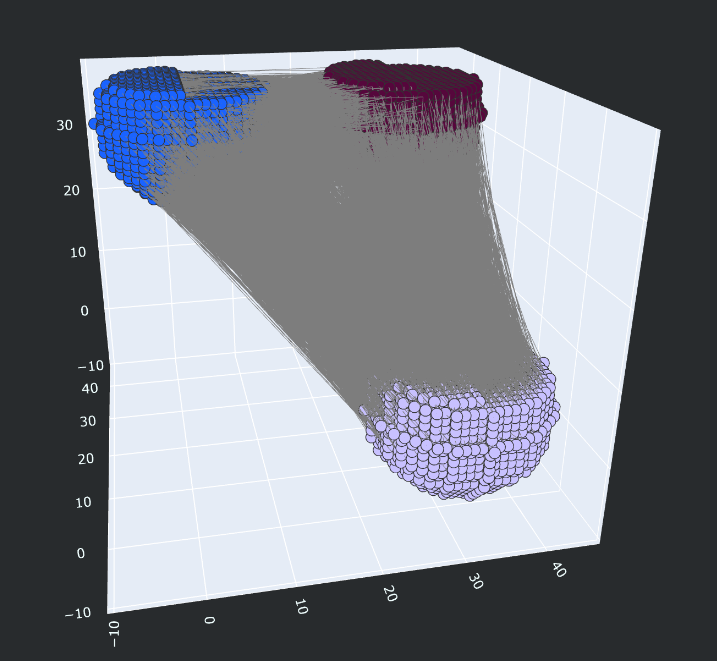
\includegraphics[width=0.5\linewidth]{images/experiment_r0_network.png}
    \caption{Structure of the network used for the $R_0$ experiments}
    \label{fig:exp_r0_network}
\end{figure}

Let $N_i$ be the number of nodes in group $i$, then the number of edges can be calculated using the following equation:
\begin{equation}
    E = \frac{n_1}{2} \cdot 5 + \frac{n_2}{2} \cdot 4 + \frac{n_3}{2} \cdot 3 + \frac{n_1+n_2}{2} \cdot 2 + \frac{n_1+n_3}{2} \cdot 2 + \frac{n_2+n_3}{2} \cdot 2
\end{equation}
It is important to note, that each edge appears in both the nodes it connects, so the number of edges is half of the sum of the degrees, which is why the number of nodes is divided by 2 in the equation. Using this equation, it can be calculated that the network contains 60,000 edges. This leads to an average amount of connections per node of $e\mu=\frac{60,000}{15,000} \cdot 2 = 8$. But the different groups must also be considered in isolation. If the $R_0$ value within a group of nodes is greater than one, the disease is likely to never die out in that group and the nodes in that group will constantly spread the disease to the other groups. An example of this is shown in the next section.

\subsection{Experiment with $R_0 < 1$}
Since this experiment uses the same network as the following experiment, which will show an example of $R_0 > 1$, the factor $e_\mu$ is static and cannot be changed. This makes $p$ the only deciding factor for $R_0$, it can be calculated using $p = \frac{R_0}{e_\mu \cdot t_I}$, so in this case with $t_I=5$ and $R_0 < 1$, $p < \frac{1}{40}$. For cases with $R_0$ close to 1, there is still a good chance that the disease will die out even if $R_0 < 1$. $p=0.024$ is chosen for an estimated $R_0=0.96$ to ensure that the disease dies out in a finite number of steps.

The parameters for the disease of this experiment are:
\begin{itemize}
    \item (vaccinated) fatality rate: 0
    \item (re-, vaccinated) infection rate: 0.024
    \item infection period $t_I$: 5
    \item initial infections: 5
    \item cure chance: 1
    \item immunity period: 0
    \item infectiousness factor: 1
\end{itemize}

Running the simulation shows that the disease is never able to spread to a large number of people and dies out after only \~9 steps. This can also be seen in the first graph of figure \ref{fig:exp_r0_small}, which shows the number of new infections per cycle. Increasing the initial number of infected nodes to 5,000 shows that even with such a large number of infections the disease still dies out after only \~40 steps

% is now able to spread to a lot of nodes intially.
% As the disease now has enough infected nodes to avoid dying out at random because of 
% randomness, it can be seen that it actually never dies out, as can be seen in the second graph
% of figure \ref{fig:exp_r0_small}. It constantly has between 50-100 new infections eveen though
% the estimated $R_0$ was only 0.96. This is due to the fact mentioned earlier, that each group
% also needs to be viewed in isolation: Group 1 has 9 connections per node so $R_0^1 = 0.02 * 7 * 5 = 1.08$
% which is bigger than 1. This means the disease has a chance to never die out within group 1 and is constantly
% spreading to the other groups from group 1.

%Lowering $p$ to 0.02 results in an $R_0=0.9$ for group 1 and a total estimated $R_0=0.8$, with these values the disease should die out in a finite amount of steps. In this case it took \~40 steps for the disease to die out, the right graph of figure \ref{fig:exp_r0_small} shows the amount of new infections up to that point.

\begin{figure*}
    \centering
    \begin{subfigure}[b]{0.475\textwidth}
        \centering
        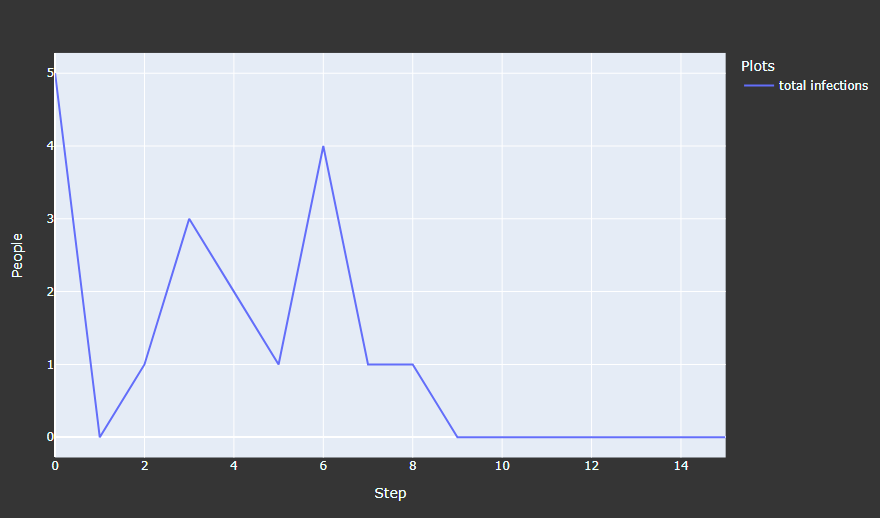
\includegraphics[width=\textwidth]{images/exp_r0_small_1.png}
        \caption[Network2]%
        {{\small Infection counts with 5 initial infections}}   
    \end{subfigure}
    \hfill
    \begin{subfigure}[b]{0.475\textwidth}  
        \centering 
        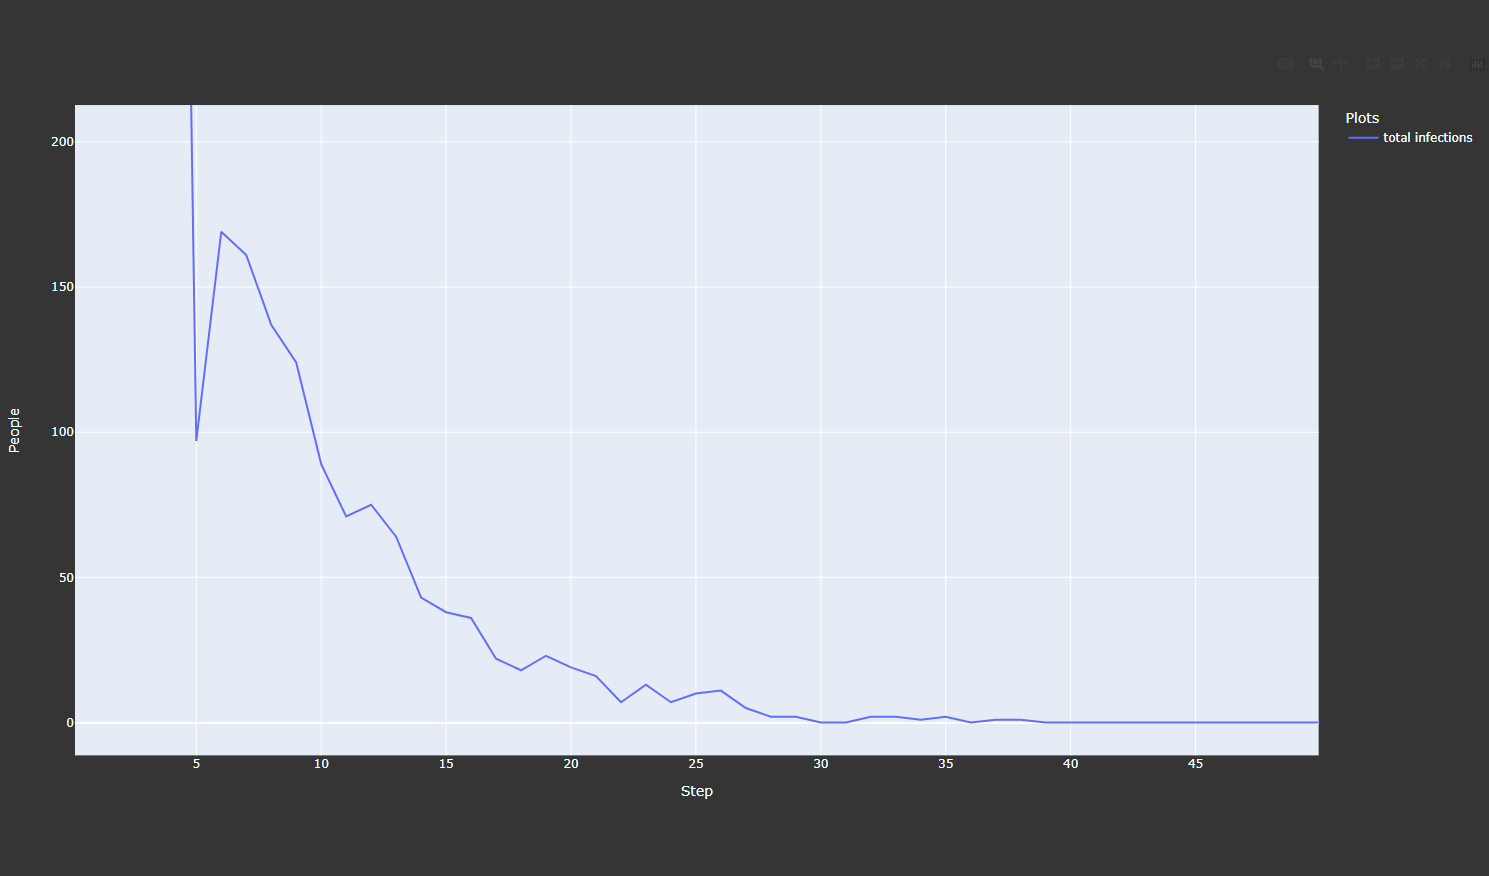
\includegraphics[width=\textwidth]{images/exp_r0_success.png}
        \caption[]%
        {{\small Infection counts with 5000 initial infections, showing that the disease
        still dies out after \~40 steps}}    
    \end{subfigure}
    \caption[ Experiment with an estimated $R_0$ of 0.96 and $p = 0.024$ ]
    {\small Experiment with an estimated $R_0$ of 0.96 and $p = 0.024$} 
    \label{fig:exp_r0_small}
\end{figure*}



This experiment supports the theory that for a $R_0 < 1$ the disease will die out in a finite amount of steps, even for $R_0$ values close to 1. 

\subsection{Experiment with $R_0 > 1$}
This experiment uses the same network as the previous one, so $p$ is again the deciding factor for $R_0$. $p = \frac{R_0}{e_\mu \cdot t_I}$ so for this case with $R_0 > 1$, $p > \frac{1}{40}$. The theory created said that it should be sufficient to have a $p$ big enough to ensure that $R_0 > 1$ in only one of the groups. Since group 1 has the most connections, $R_0^1 > 1$ if $p > \frac{1}{9\cdot5} = 0.0222$. Since the closer $R_0$ to 1, the higher the chance that the disease will randomly die out, $p=0.03$ is chosen, resulting in a $R_0^1 = 1.35$ and $R_0 = 1.2$, where $R_0^1$ is big enough for the disease to have a decent chance of surviving indefinitely.

The properties that were changed from the previous experiment are:
\begin{itemize}
    \item (re-, vaccinated) infection rate: 0.032
    \item initial infections: 50
\end{itemize}

Running the simulation shows that the disease consistently dies out at about 70 steps. The left graph in figure \ref{fig:exp_r0_big} shows the number of infections. The expectation was that the disease would have a decent chance of surviving, but even after 50 attempts it never survived. This can be explained by the network structure: the nodes in group 1 have 9 connections, but 4 of them are "worth less" because the nodes it can spread to in the other groups are not able to spread the disease to another 9 new nodes, but only 7 or 8 depending on the group. This means that when calculating $R_0$, the nodes in group 1 cannot be considered to have 9 connections, somewhere around 8 would be more accurate. This makes $R_0^1 = R_0 = 1.2$ which is not high enough for a decent chance of indefinite survival. This shows how difficult it can be to calculate $R_0$ in complex networks, because there is no formula that can take the network structure into account.

Increasing $p$ to 0.036 is enough to make the disease live indefinitely with $R_0 = 1.44$. After running the simulation for 20,000 cycles, the disease is still alive and infecting new nodes. This supports the theory that with $R_0 > 1$ there is a probability $> 0$ that the disease never dies out. Another option is to increase the connections within group 1, which increases $R_0^1$ so that the disease is able to survive within group 1. This again shows that in addition to viewing the network as a whole, each part of the network must also be viewed in isolation. If the disease is able to survive in a subset of the network, it will never die out and will constantly spread to other parts of the network, even though it would never be able to survive in the other parts of the network.


\begin{figure*}
    \centering
    \begin{subfigure}[b]{0.475\textwidth}
        \centering
        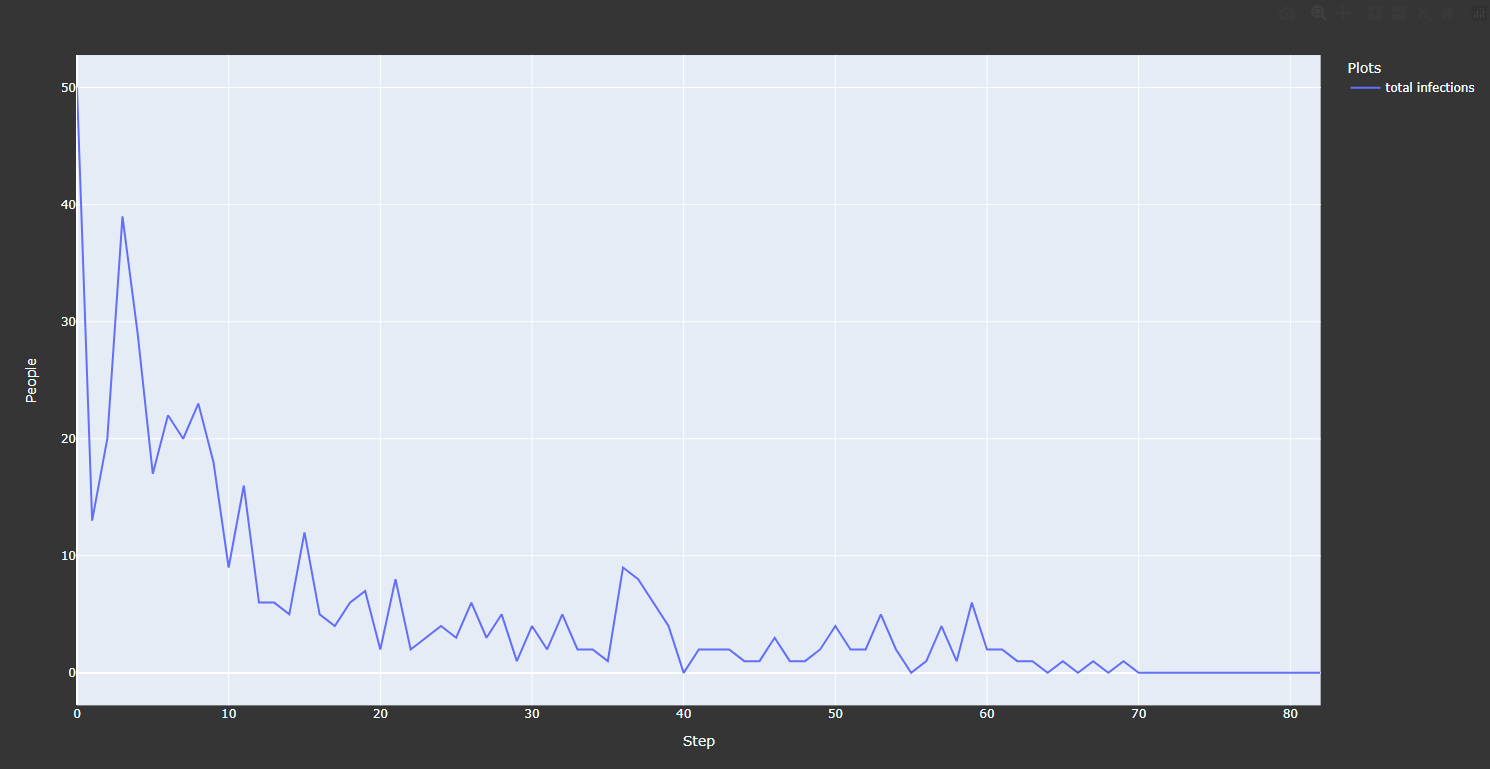
\includegraphics[width=\textwidth]{images/exp_big_r0_fail.png}
        \caption[Network2]%
        {{\small Infection counts with 50 initial infections, $R_0=1.2$ and $p = 0.032$.}}   
    \end{subfigure}
    \hfill
    \begin{subfigure}[b]{0.475\textwidth}  
        \centering 
        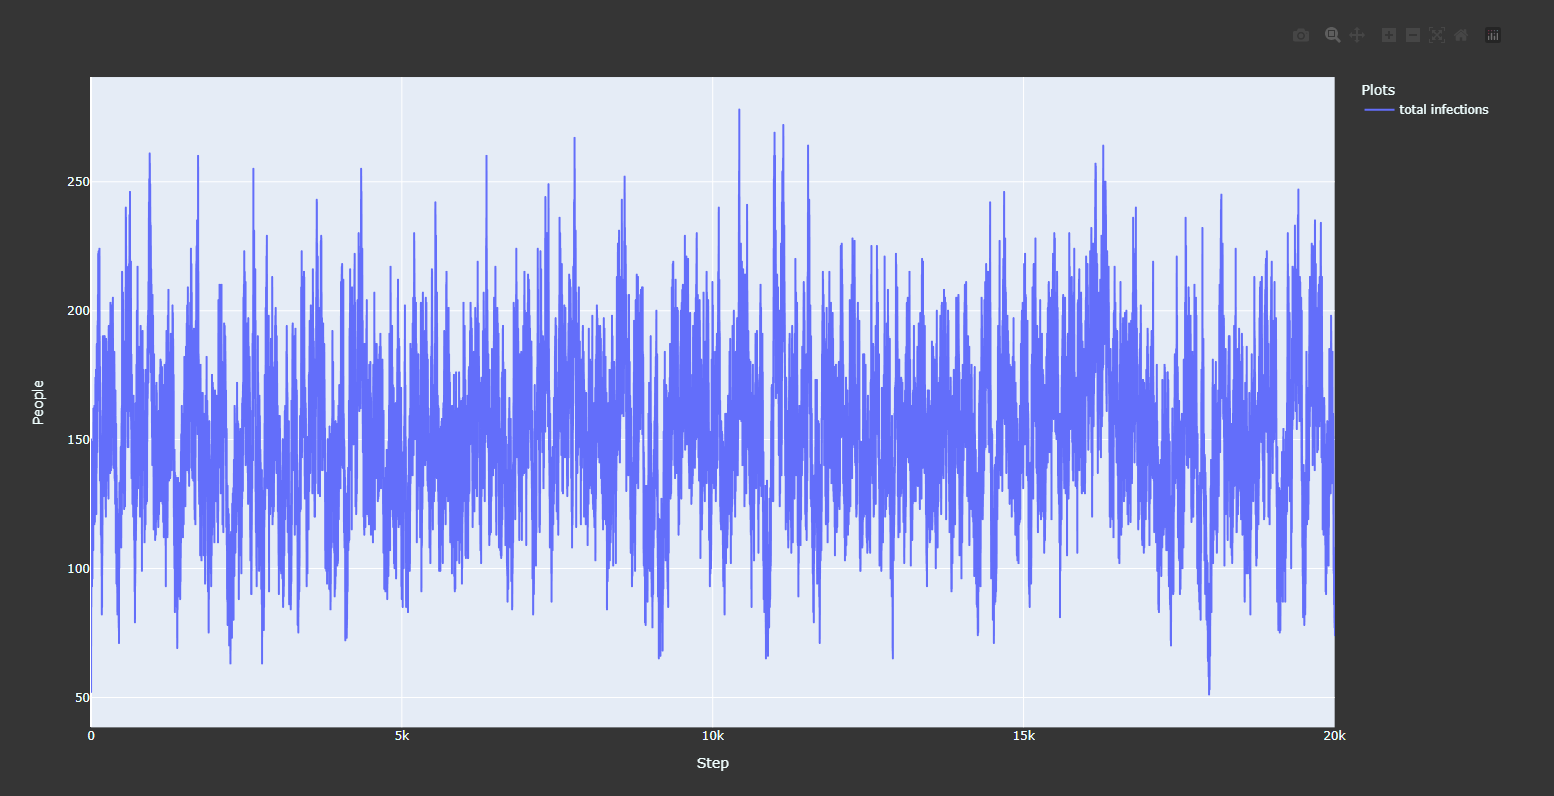
\includegraphics[width=\textwidth]{images/exp_big_r0_success.png}
        \caption[]%
        {{\small Infection counts with 150 initial infections, $R_0=1.44$ and $p = 0.036$}}    
    \end{subfigure}
    \caption[Experiment with an estimated $R_0$ of 0.64 and $R_0^1 = 1.12$]
    {\small Experiment showing that diseases with $R_0$ close to 1 still have a decent chance of dying out. Although it is theoretically possible even for the disease with $R_0$ to survive indefinitely, it is statistically improbable because the chance it dies out each cycle is too big.} 
    \label{fig:exp_r0_big}
\end{figure*}

\subsubsection{Changing the network}
To prove the above assumption that the network structure does have an effect on $R_0$, this experiment uses the same disease as the previous one with $p=0.036$ and 150 initial infections. The network will have only half as many edges, group 1 has 2 intra-group connections for each node, group 2 has 2 and group 3 has 2 intra-group connections. Between each pair of groups there is 1 connection per node. This new network has 30,000 edges, resulting in $e_\mu$ = 4. Thus the new estimated $R_0=2\cdot0.375=0.75$ which is smaller than 1 so the expectation is that the disease will die out even though it has the same infection rate as before.

After 20 cycles, the disease has died out, supporting the theory that the network structure, and thus $e_\mu$, has an effect on the spreading of diseases and the value $R_0$. Graph \ref{fig:exp_change_network} shows the number of infections until the disease died out.

\begin{figure}
    \centering
    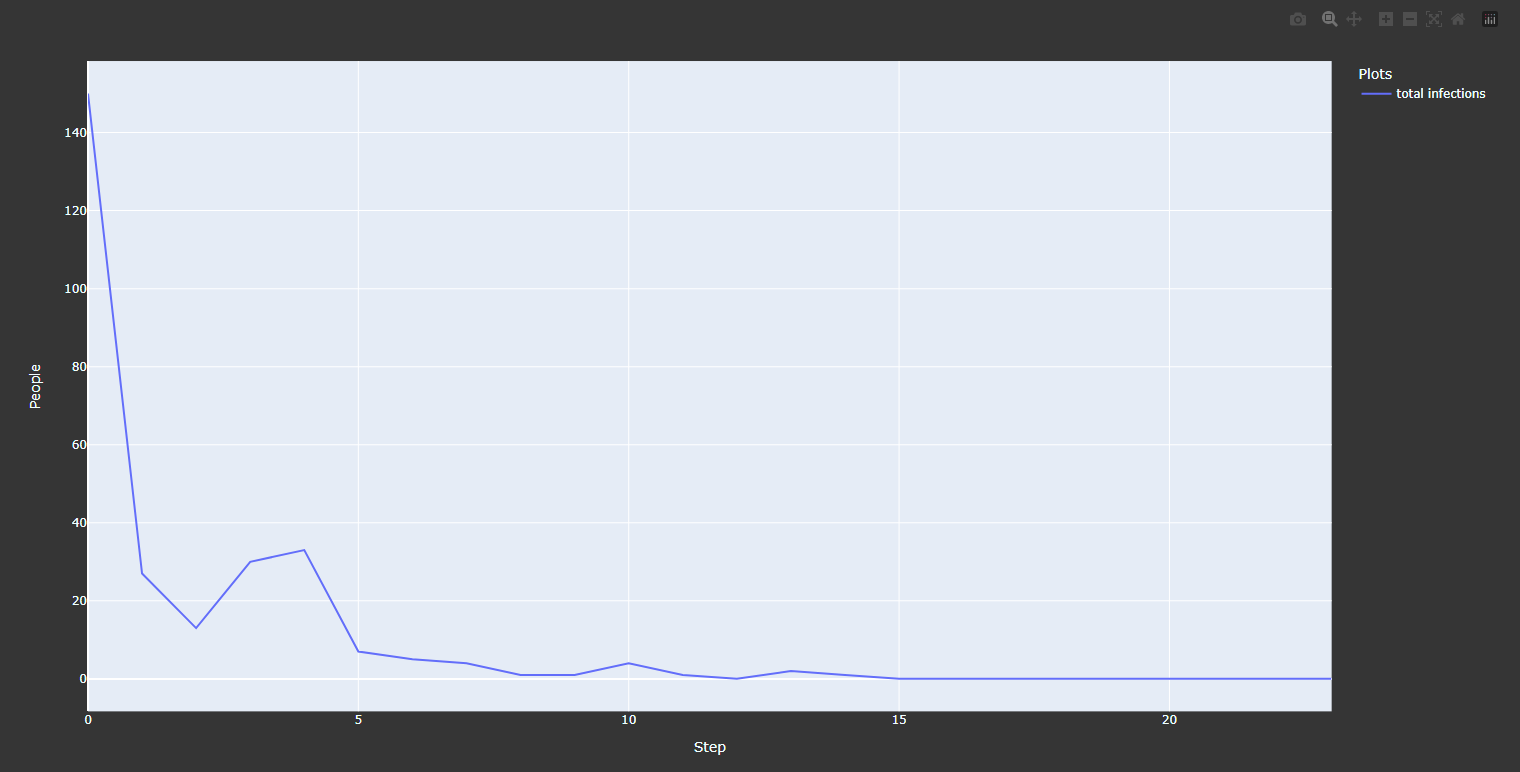
\includegraphics[width=0.5\linewidth]{images/exp_changed_network.png}
    \caption{Amount of infections with the same diseases ($p = 0.036$) but a network with half as many connections}
    \label{fig:exp_change_network}
\end{figure}

To support the theory from earlier that each group must also be viewed in isolation when calculating $R_0$, the network is changed again. Group 1 has 8 intra-group connections for each node, group 2 has 1 and group 3 has 1 intra-group connection. Between each pair of groups there is 1 connection per node, for a total of 40,000 edges, giving $e_\mu=5.\overline{3}$ and $e_\mu^1=8$ for connections within group 1. The same $p = 0.036$ is used, resulting in $R_0 = 0.96$ while $R_0^1 = 1.44$. Running the simulation again shows that even though $R_0 < 1$ the disease manages to survive indefinitely. $R_0^1 = 1.44$ means that the disease has a chance of never dying out within group 1 and is constantly spreading from group 1 to the other groups. Figure \ref{fig:exp_subgroups} shows the number of infections per group. Group 1 has significantly more infections and keeps the disease alive, while groups 2 and 3 have similar, lower amounts of infections. This experiment shows how difficult it is to estimate $R_0$ for complex networks, as the network may contain highly connected subgroups where the disease can live longer and spread to the rest of the network again.

\begin{figure}
    \centering
    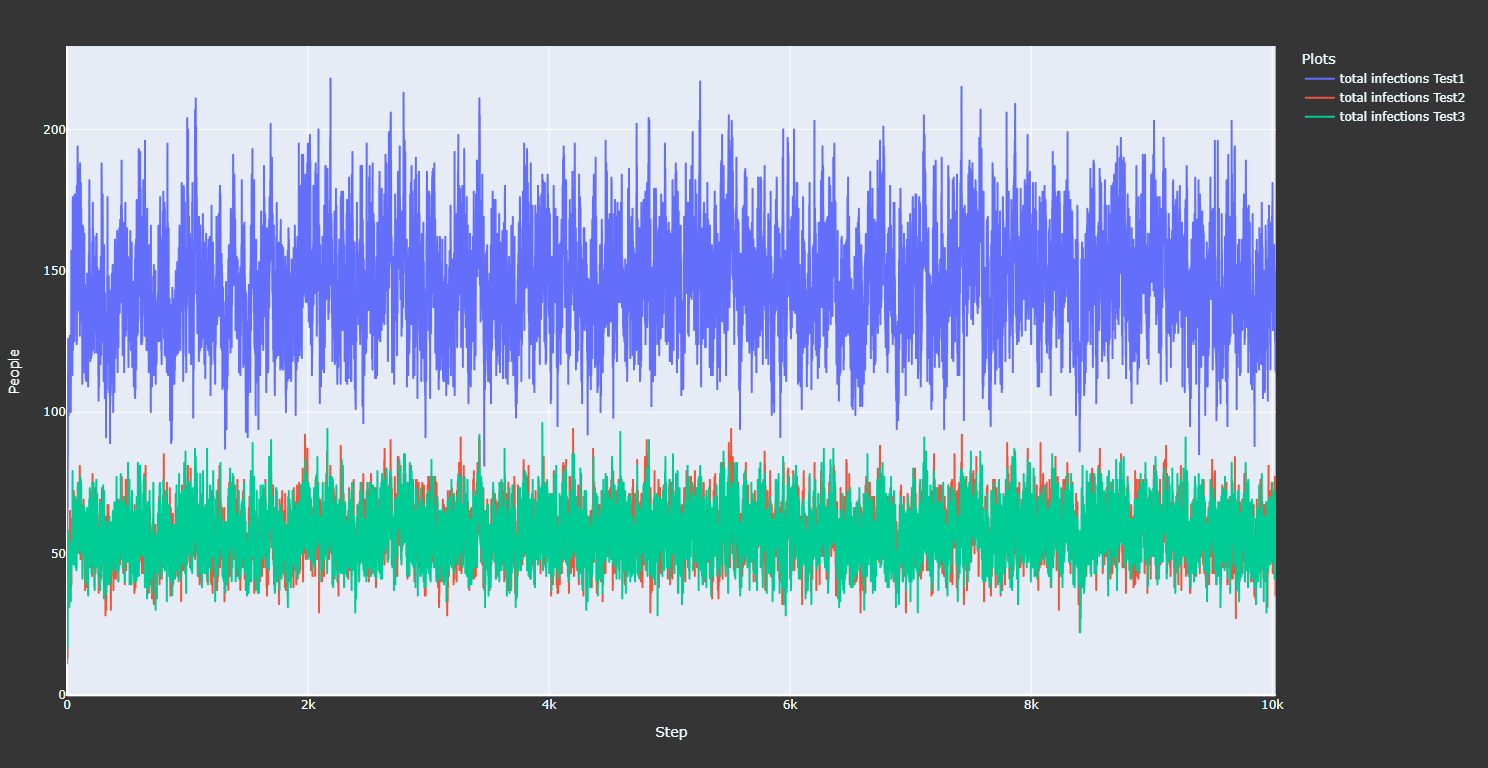
\includegraphics[width=0.5\linewidth]{images/exp_subgroups.png}
    \caption{Infections per group with $p = 0.036$ and $R_0 = 0.96$, the disease never dies out}
    \label{fig:exp_subgroups}
\end{figure}


\section{Multiple Diseases}
Interesting dynamics can be observed when multiple diseases are introduced into the same social network. Cases with two diseases, where one or both of the diseases have a $R_0 < 1$, do not present an interesting scenario, since once one disease has died out, the problem is reduced to one disease. But if both (or more) diseases have a $R_0 > 1$, then they will compete against each other for survival, assuming that a person can only be infected by one diseases at a time, e.g. because they stay at home until they are cured, so they cannot be infected by another disease during that time. Since a disease must constantly infect new nodes to stay alive, the diseases can wipe out other diseases by infecting all the nodes themselves, leaving no nodes available to infect for other diseases.

For diseases with a similar $R_0$, the two diseases will each have \~50\% of infections. Now consider a case where one disease $d_1$ has $R_0^1=5$ and the second $d_2$ has $R_0^2=2$. Looking at the diseases in isolation, both are theoretically able to survive, since both $R_0^1 > 1$ and $R_0^2>1$. Looking at the situation where both diseases are in the same network, $d_1$ will infect significantly more people than $d_2$, about 2.5 times as many. This means that $d_1$ will have $~\frac{5}{7}$ of the total infections during the first wave. Since $d_1$ has many more infected nodes during the first wave, that makes it even easier for it to spread than $d_2$. At the boundaries where susceptible nodes have connections to nodes infected with $d_1$ and also to nodes infected with $d_2$, $d_1$ will infect $\frac{5}{7}$ of those nodes. This will slowly reduce the number of nodes infected with $d_2$ until none are left and $d_2$ has died out, even though its $R_0^1>1$. This means that in networks with more than one disease, the one  with the highest $R_0$ value is the most likely to survive.

\subsection{Experiment}
This theory can again be supported by conducting an experiment using the developed simulation tool. The network will be the same as in the previous experiment, consisting of 3 groups with more intra-group connections than inter-group connections. The exact structure is explained in section \ref{sub:exp_network}.

Two diseases are used for this simulation:
\begin{itemize}
    \item (vaccinated) fatality rate: 0
    \item (re-, vaccinated) infection rate: 0.06 for Disease 1 / 0.04 for Disease 2
    \item infection period $t_I$: 5
    \item initial infections: 50
    \item cure chance: 1
    \item immunity period: 0
    \item infectiousness factor: 1
\end{itemize}

First, the experiment is run with the two diseases separately to show that they never die out on their own. The results can be seen in figure \ref{fig:exp_multiple_diseases_individual}, which shows the number of new infections up to cycle 5000, indicating that the individual diseases have not died out by then.

\begin{figure*}
    \centering
    \begin{subfigure}[b]{0.475\textwidth}
        \centering
        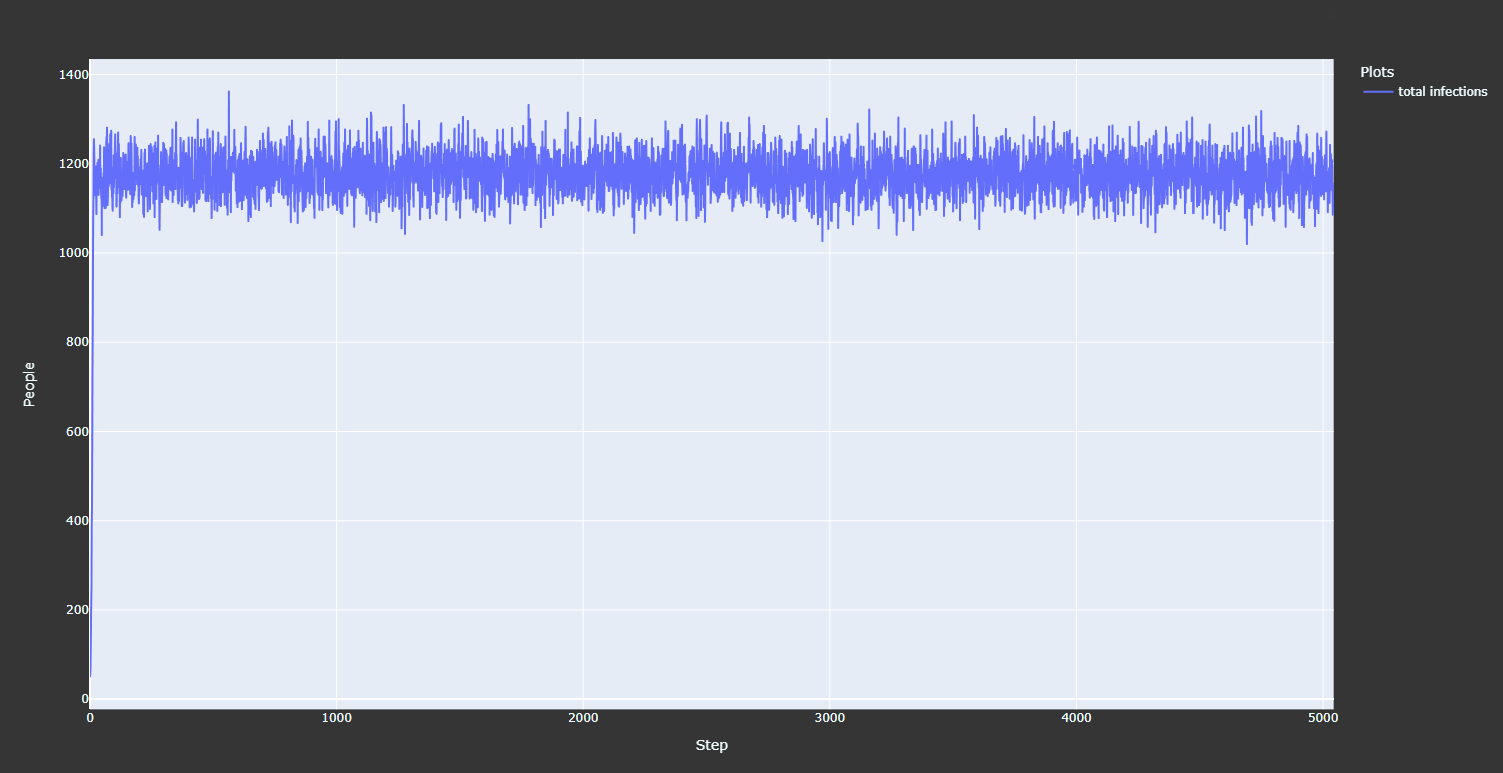
\includegraphics[width=\textwidth]{images/exp_multiple_diseases_d1.png}
        \caption[Network2]%
        {{\small Infection counts for disease 1 with 50 initial infections and $p = 0.06$}}   
    \end{subfigure}
    \hfill
    \begin{subfigure}[b]{0.475\textwidth}  
        \centering 
        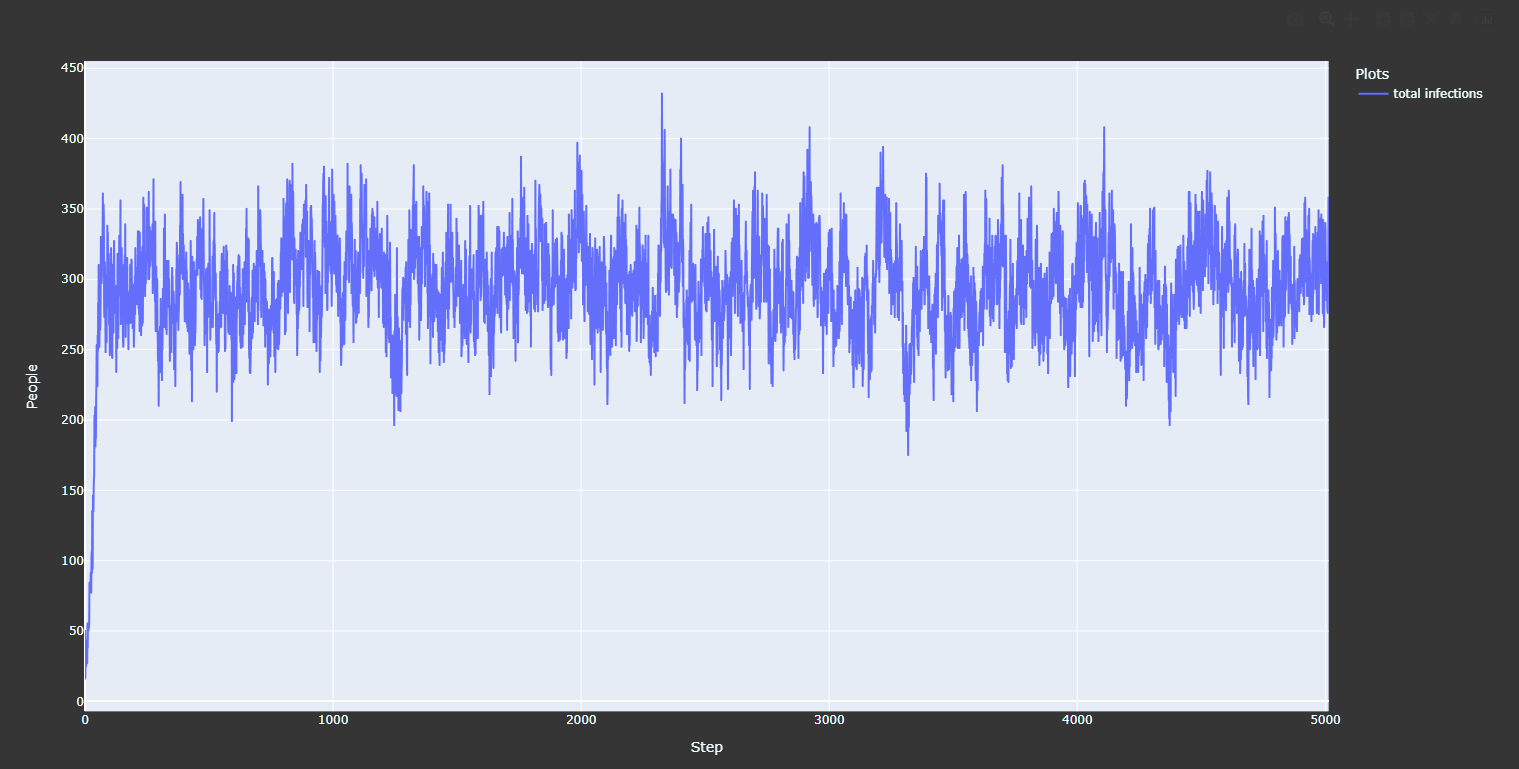
\includegraphics[width=\textwidth]{images/exp_multiple_diseases_d2.png}
        \caption[]%
        {{\small Infection counts for disease 2 with 150 initial infections and $p = 0.04$}}    
    \end{subfigure}
    \caption[Experiment to show both diseases never die out on their own]
    {\small Experiment to show both diseases never die out on their own} 
    \label{fig:exp_multiple_diseases_individual}
\end{figure*}

Now both diseases are used simultaneously. After 40 cycles, $d_2$ has died out because the new infections of $d_1$ have increased so much that there are not enough nodes available for $d_2$ to infect. This increase in infections with $d_1$ and decrease in infections with $d_2$ is shown in figure \ref{fig:exp_multiple_diseases}.

\begin{figure}
    \centering
    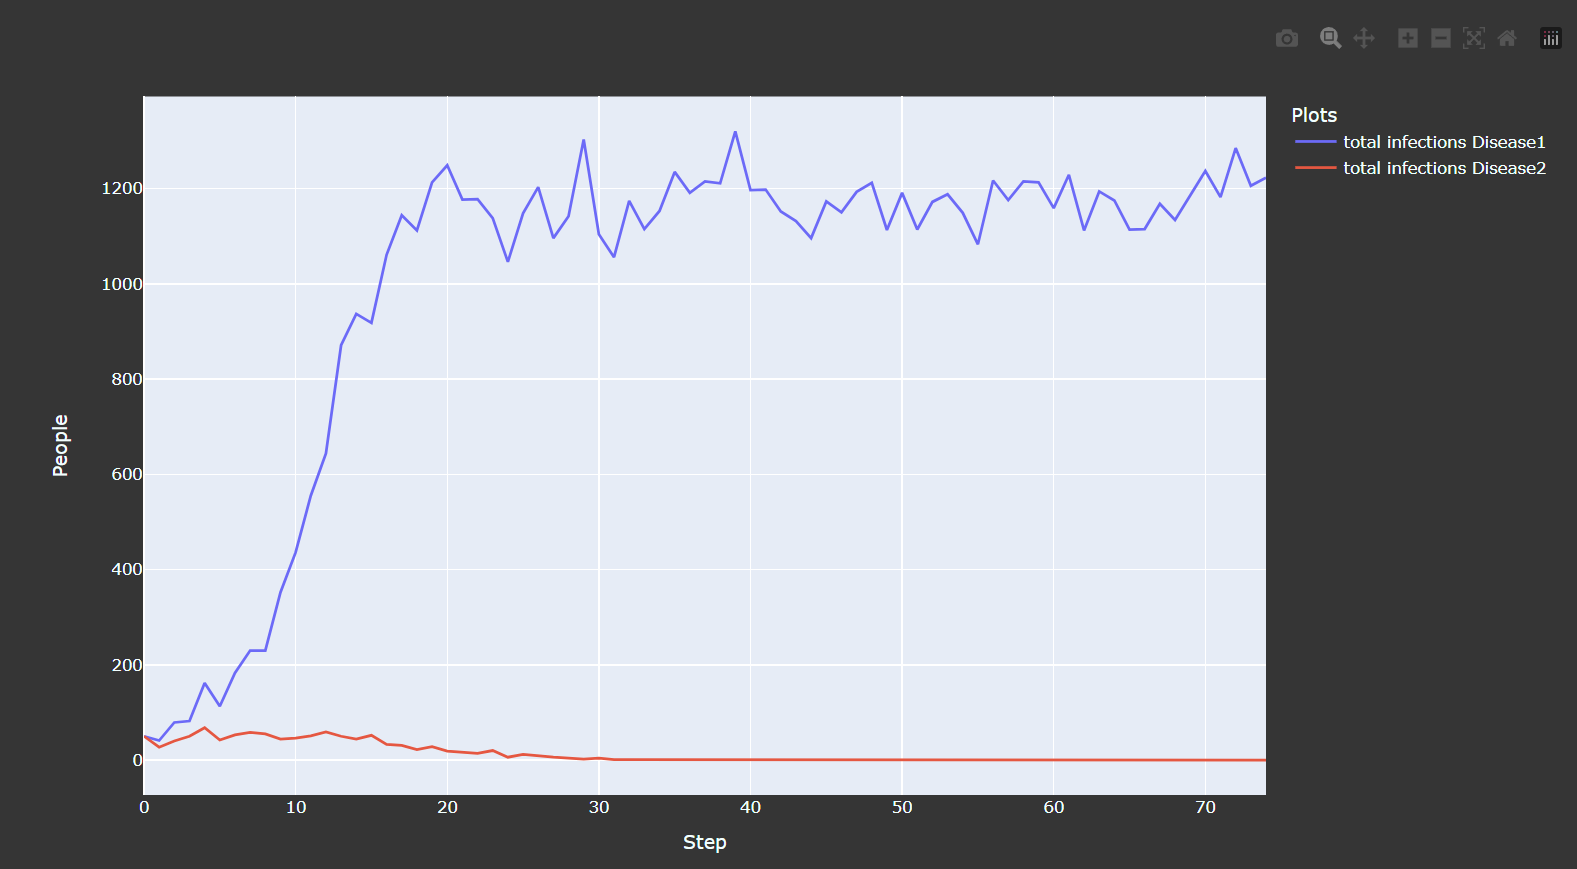
\includegraphics[width=0.5\linewidth]{images/exp_multiple_diseases_both.png}
    \caption{Infections per disease with $p = 0.06$ and $p = 0.04$, disease 2 dies out after 40 steps even though it did not die out when the two diseases were simulated in isolation}
    \label{fig:exp_multiple_diseases}
\end{figure}

This supports the theory that in networks with multiple highly infectious diseases the one with the highest $R_0$ value is the one most likely to survive.

\section{Small-World Phenomenon}
The small-world phenomenon is also known as six degrees of separation. The theory is that in an arbitrarily large social network the length of the path from one person to any other person is, on average, only 6 steps. To support this theory, Stanley Milgram conducted an experiment in the 1960s \cite{smallWorld}. In this experiment, Milgram gave a letter to a random source person in Nebraska, USA, and told them to deliver it to a target person in Massachusetts, USA. The source person was given only basic information about the target, such as address and occupation and each person was allowed to send the letter only to someone they knew on a first-name basis, with the goal of getting the letter closer to its target. Each person in the chain was given the same information. After many iterations of this experiment, the average number of persons it took to deliver the letter to its target was between 5 and 6 persons, hence the name of the \textit{Six Degrees of Separation} principle.

This experiment does not always find the shortest path, because people forward the letter only to the person they think is closest to the target. Unknown to them, there may be another person they know who is much closer to the target, making for a shorter path that is never discovered. To find the true shortest path, each participant would have to forward the letter to all of their friends, keeping track of which path the letter took. Then, when all letters have arrived at the target, the true shortest path is that of the letter that required the least number of people to arrive.

\subsection{Experiment}
For this experiment a network with only one group is created. This group contains 10,000 nodes, with each node having 6 connections. Although this network is not completely accurate to a real situation. Usually a person's network of friends is tightly coupled, a person's friends usually know each other and their friends know the original person etc. Also, a person tends to know more people who live in an area close to them and fewer people who live farther away. This leads to a highly connected network with only short connections and a few random longer connections. The network used for this experiment uses only random edges, which does not represent the fact that the geographically closer people are, the more connections they have. However in the current day, the internet allows for many more long-distance connections, which makes the used network used more valid in this context.

\begin{figure}
    \centering
    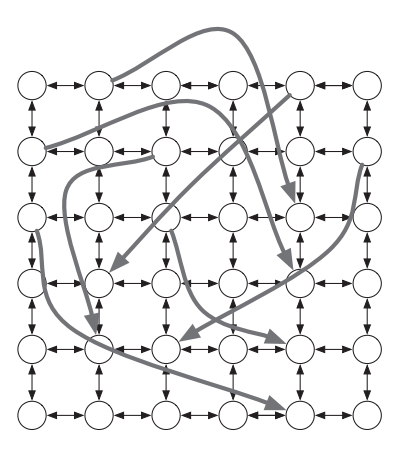
\includegraphics[width=0.5\linewidth]{images/sw_true_network.png}
    \caption{True structure of a network showing the friends of persons. The
    geolocically closer people are the higher the amount of connections. There
    are only few connections over longer range. (source: \cite{networks})}
    \label{fig:oscillation}
\end{figure}


To show that each node can be reached in only six steps, a disease with an infection rate of 1 and an infection duration of 1000 is used. Initially, only one node is infected. Figure \ref{fig:small_world_network} shows the network after 6 cycles.

\begin{figure}
    \centering
    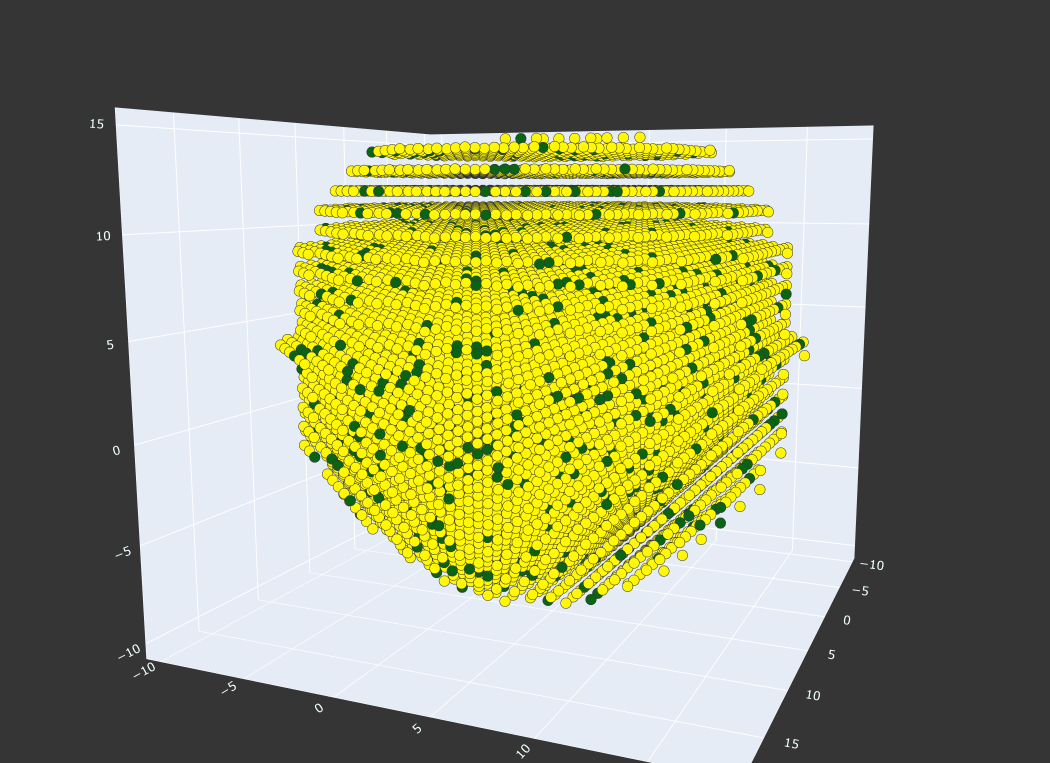
\includegraphics[width=0.5\linewidth]{images/small_world_network.png}
    \caption{Network after 6 cycles, yellow nodes have a shortest connection with 6 or less steps to the starting node,
    green ones have a shotest connection with more than 6 edges to the starting node}
    \label{fig:small_world_network}
\end{figure}

After cycle 7, all nodes are infected, i.e. they could all be reached from the starting node in a maximum of 7 steps. The exact numbers of new infections per step are: 6, 30, 150, 717, 2893, 5306 and 897. Using these values, the average shortest path length can be calculated, which is \~5.5964. This coincides with the findings of Milgram \cite{smallWorld}, whose experiments showed that the average length is somewhere between 5 and 6.

To reduce the limitation of the used network in terms of random connections, another network structure could be used. This more closely models the existence of highly connected local friend groups, where everyone knows each other and a few random connections to people from other friend groups that are farther away. This network uses a large number of groups with relatively few members each. In this case, 100 groups of 5-10 people are used, where each node is connected to 4 others of the same group and each group of people is connected to 3-4 other groups, with only 0-1 edges per node. This again results in a network where each node has an average of 6 connections.

The same disease is used in this network and the state of the network after cycle 6 can be seen in figure \ref{fig:small_world_groups}.

\begin{figure}
    \centering
    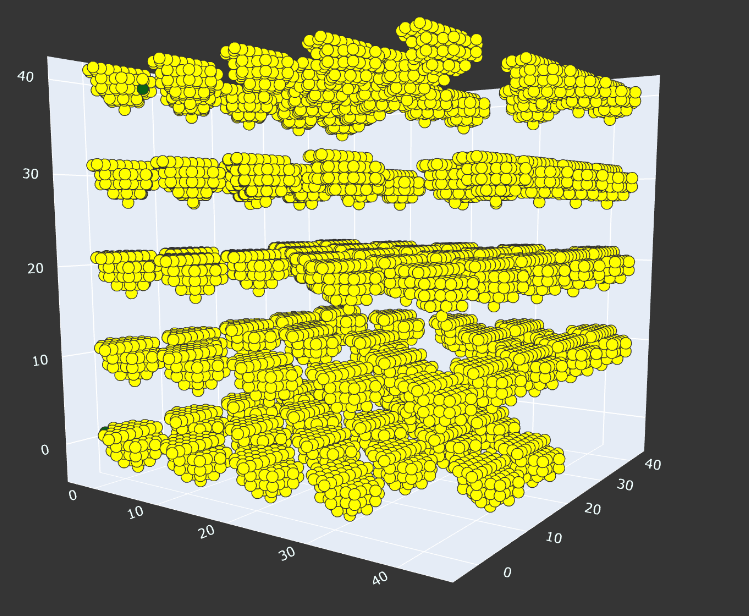
\includegraphics[width=0.5\linewidth]{images/small_world_groups.png}
    \caption{Network after 6 cycles, yellow nodes have a shortest connection with 6 or less steps to the starting node,
    green ones have a shotest connection with more than 6 edges to the starting node}
    \label{fig:small_world_groups}
\end{figure}

This shows that in this network it is also possible to reach all other nodes in only six steps, even though there are only a few long-distance connections and a lot of tightly coupled small groups. The average path length in this experiment was \~5.6621.


